\chapter{Deep Learning}

Deep Learning (DL) is a subfield of Neural Networks (NN) which in turn is a subfield of Machine Learning (ML) which again is a subfield of Artificial Intelligence (AI). Figure \ref{fig:MLOverview} shows a Neural Network relevant taxonomy of AI. There are many advantages of ML over more traditional statistical methods as often found in statistical learning. Some of them are that ML does not require any hypothesis and deep understanding of the underlying data. While statistical learning is mostly about inference (deducing properties of an underlying probability distribution, sampled from a larger population), ML is mostly about predictions in supervised, unsupervised and semi-supervised learning. It also does not operate on assumptions like normality, multicollinearity and homoscedasticity etc.. Statistical Learning operates on much smaller datasets with only a few attributes and therefore is less fit for problems with millions of possible and possibly unknown attributes and data samples. Machine Learning excels at identifying patterns from large datsets through iterations and being able to predict or classify previously unseen data.
Traditional Machine Learning approaches were based on very specific feature extractions that needed to be found/created manually and could take months to fine tune. The biggest downside was that the features often were not generalizable but were very domain specific. Even looking at the same object from different angles or from different photographs often needed additional fine tuning of existing features or creating new ones. Some of the feature extraction algorithms include Scale Invariant Feature Transform (SIFT), Histogram Oriented Gradient (HOG), Local Binary Pattern (LBP). Learning algorithms that are applied on these features are e.g.: Support Vector Machines (SVM), Random Forest (RF), Principal Component Analysis (PCA), Kernel PCA (KPCA), Linear Decrement Analysis (LDA), Fisher Decrement Analysis (FDA) and many more \ref{fig:MLOverview}. New Machine Learning methods are able to automatically learn feature representations which is much less labor intensive and often very surprising as features are learned that don't intuitively make sense [TODO: show some examples] but perform really well, but sometimes things are learned that correlate with the provided labels but have no causality [TODO: some counter examples].

\begin{figure}[H]
  \centering
  \caption{Partial taxonomy of Artificial Inteligence \cite{alom2018history}}
  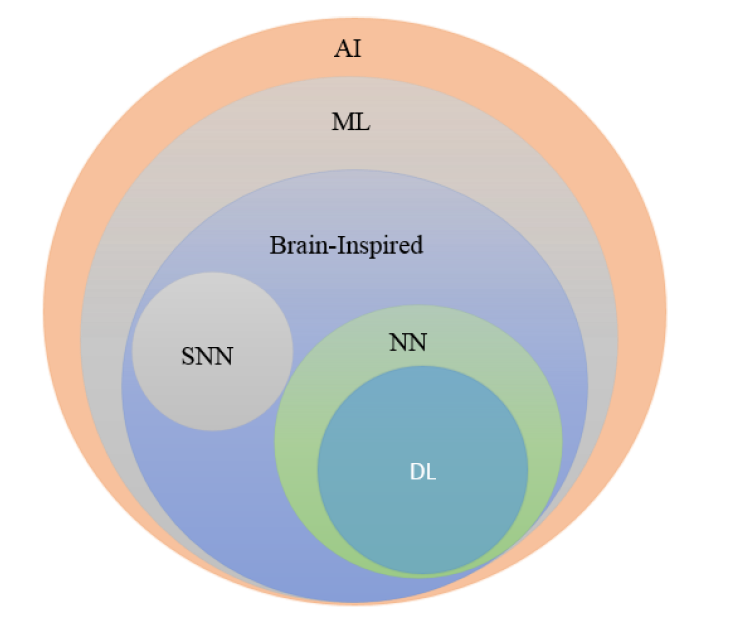
\includegraphics[scale=0.4]{chapter3/MLOverview}
  \label{fig:MLOverview}
\end{figure}

An Artificial Neural Network (ANN) tries to mimic the behavior of the human brain to a primitive extent. The analogy of the artificial neuron helps to understand the parallels between how biological neurons pass information but it is only an analogy and therefore should be used very cautiously. There are more differences than similarities and the human brain is still in many aspects a mystery to be solved. Nonetheless the abstract notion of a neuron is visually very appealing and useful. Figure \ref{fig:Neurons} show on the left side a biological neuron with all its relevant parts and the mathematical representation of it on the right side. The biological neuron receives its inputs from other neurons through its dendrites (through many different neurotransmitters in the synapses). If a certain threshold is reached in the cell body from all its dendrites, it transmits the information along the axon to other neurons. The axon branches out at the and reaches several different neurons and the process continues. Learning is believed to happen when the sensitivity of the synapses changes and new pathways are formed through branching the axon and connecting to new axons or making the current pathways stronger.

\begin{figure}[H]
  \centering
  \caption{A biological neuron on the left versus the mathematical representation of neuron how it is used in neural networks on the right. \cite{cs231neuralnetworks}}
  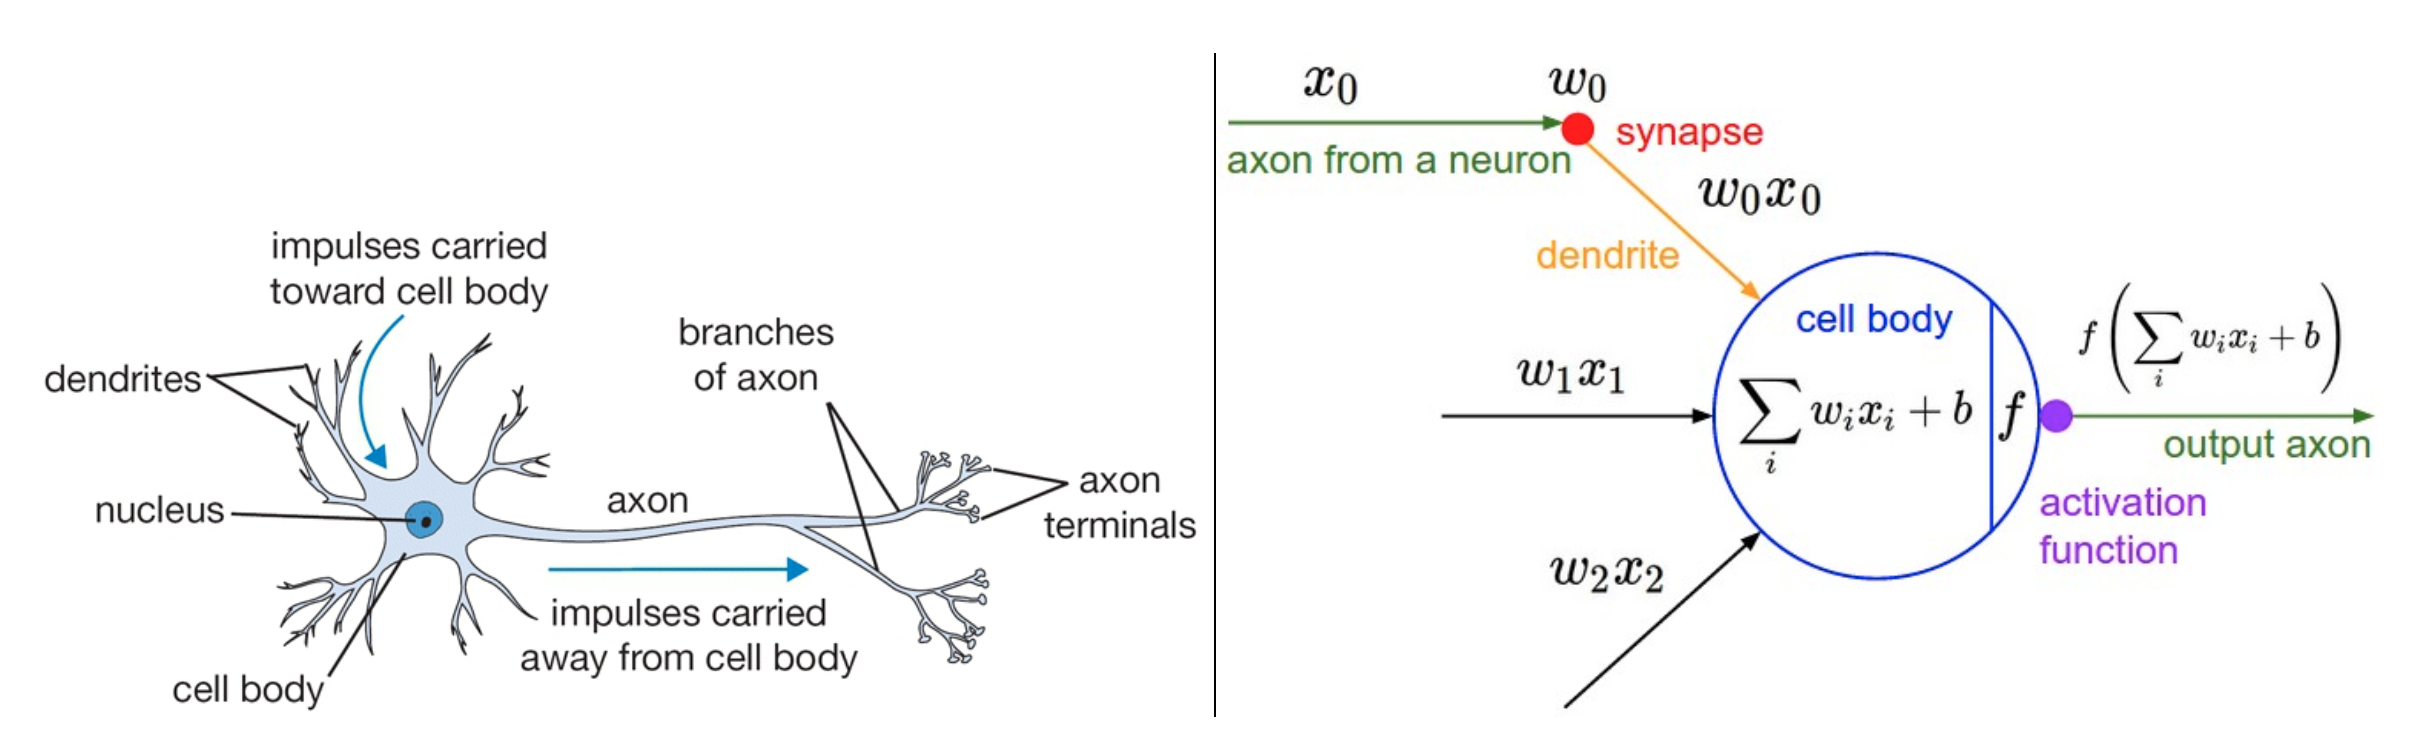
\includegraphics[scale=0.35]{chapter3/Neurons}
  \label{fig:Neurons}
\end{figure}

This is indeed similar to how an artificial neuron processes information and passes it forward. An artificial neuron receives inputs (e.g. $x_0$) from other neurons and applies a weight matrix (e.g. $w_0$) and a bias (e.g. $b$) on it. The weights and biases can be compared to the strength of the synapses in the biological neuron and these can be changed through learning. Actually that's what happens during the backpropagation explained later on. The weights are adjusted in order to classify the input more accurately. In the cell body of the mathematical representation performs a dot product between the inputs and the weights adds the bias ($w_i x_i + b$) and then applies some kind of activation function. This activation function needs to be non-linear, because otherwise all the matrix computations of different neurons could be collapsed into one linear computation and no learning would take place. Just a linear regression would be achieved.
Traditionally a sigmoid function has been used for the activation function since it takes any real number as inputs and outputs numbers between 0 and 1. That is a very intuitive non-linearity function to work with but has some disadvantages when backpropagating the loss function and adjusting the parameters in the weight matrices.  During backpropagation the loss is computed according to some loss function and then back propagated through all layers and units. During that process the partial derivatives of the loss function are computed with respect to the input variables (e.g. $x_i^j$) of that specific unit. In the used notation the superscript denotes the layer whereas the subscript denotes the unit. These derivatives are then multiplied by a learning rate alpha and added to the current weights. This process of changing the weights towards a optimal loss is called learning and happens through many iterations. In Figure \ref{fig:SigmoidTanh} the two activation functions, the sigmoid and the tanh, are shown. Since the partial derivatives are crucial in learning - the stepper the derivation the bigger the change in weights - the disadvantages of both non-linearties are clearly visible towards the borders. If the function moves mostly horizontally, the first derivation will be near 0 thus learning happens very slow. The tanh has a much steeper function around the center (leading to a bigger first derivative) but still has the same problem towards the borders.

\begin{figure}[H]
  \centering
  \caption{The sigmoid non-linearity takes in any real number and outputs a number in the range [0,1], wheras the tanh non-linearity takes the same input but outputs a number in the range of [-1,1]. \cite{cs231neuralnetworks}}
  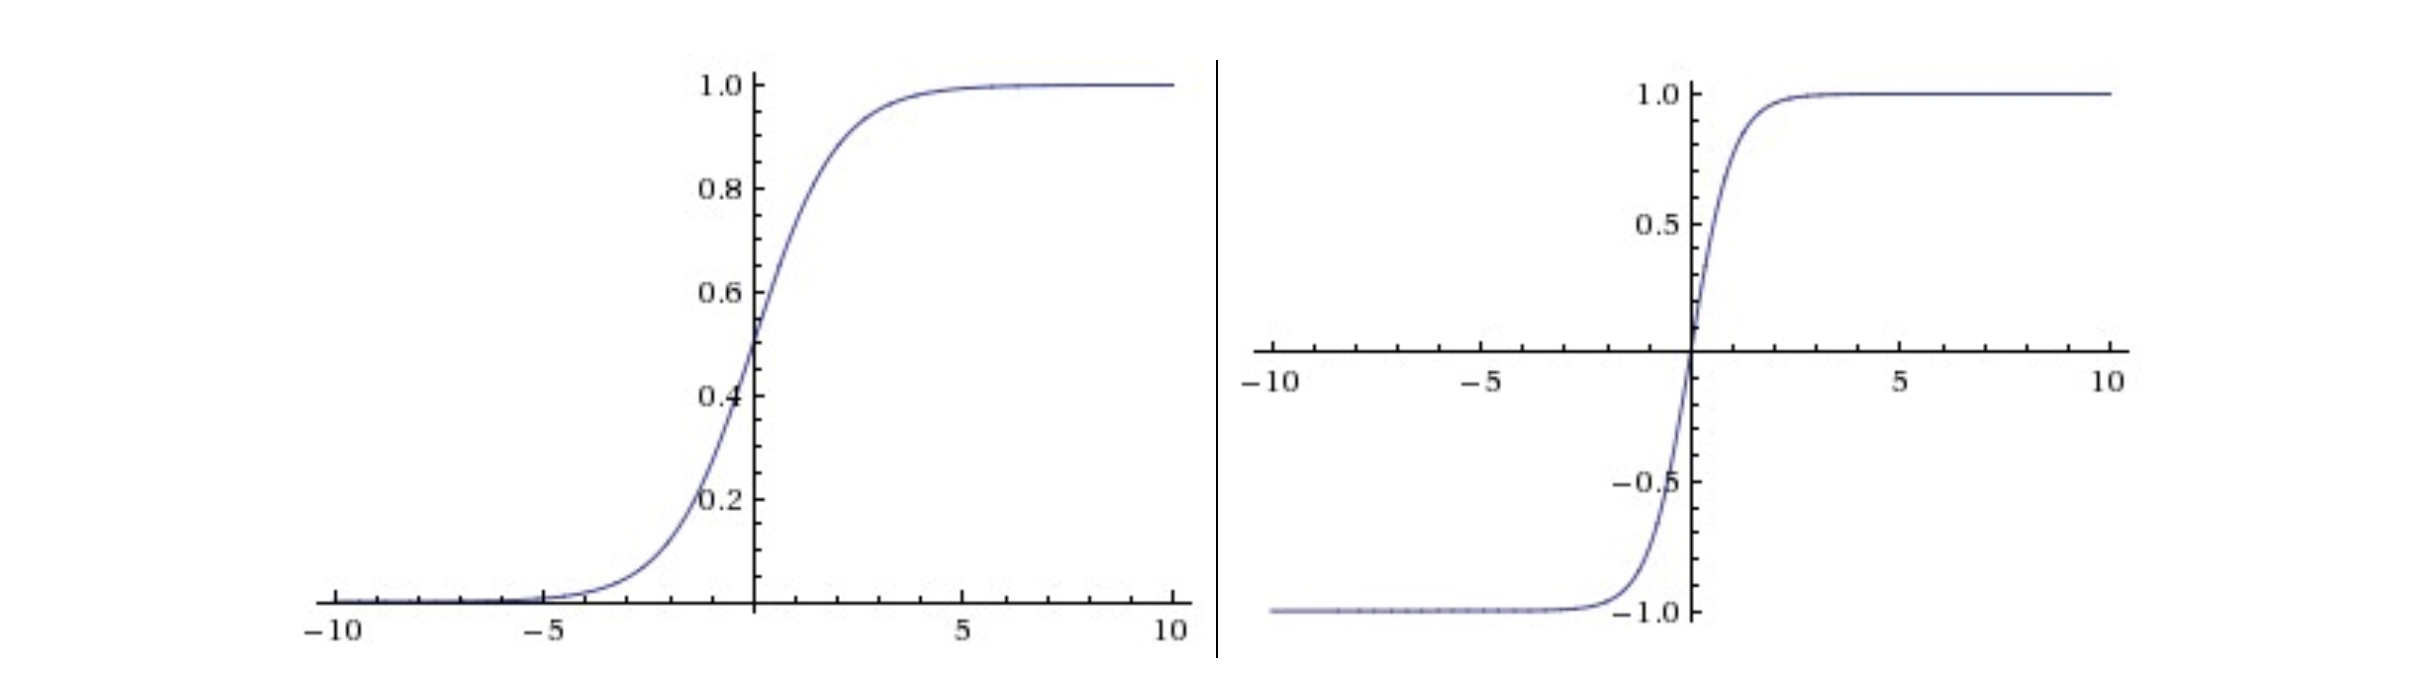
\includegraphics[scale=0.35]{chapter3/SigmoidTanh}
  \label{fig:SigmoidTanh}
\end{figure}

For the above mentioned reasons, the sigmoid non-linearity is not used anymore except in the last layer and only if the task is a binary classification. For that special case the sigmoid is still a valid function. As an alternative the Rectified Linear Unit (ReLU) is used. It is very simple, fast to compute and easy to back-propagate since the derivatives are 0 or a fixed value. In order to omit the deactivation of units, which happens if the input values are smaller than 0, a leaky ReLU can be used. Both non-linearities can be seen in Figure \ref{fig:ReLU}.

\begin{figure}[H]
  \centering
  \caption{Rectified Liner Unit on the right side. Deactivating units if their input values are negative. Leaky ReLU that never deactivates units. \cite{reinventingNN}}
  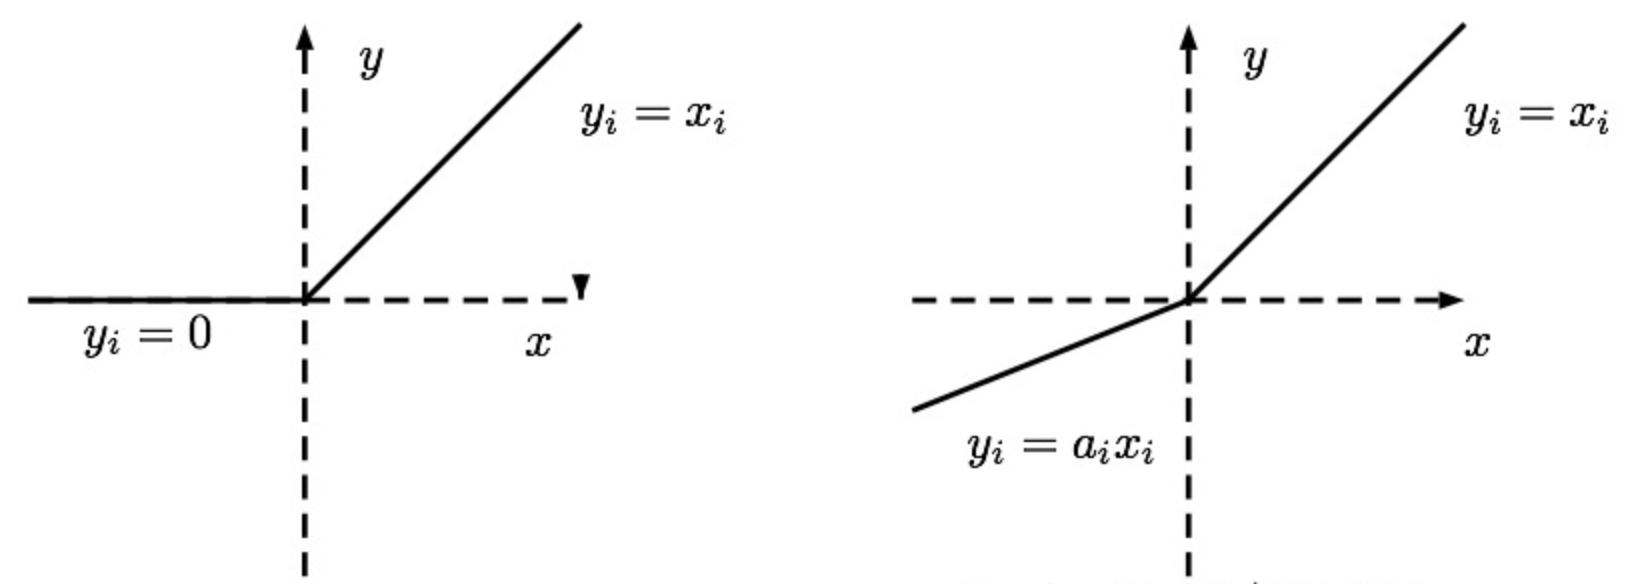
\includegraphics[scale=0.35]{chapter3/ReLU}
  \label{fig:ReLU}
\end{figure}

The components of an Artificial Neural Network (ANN) are the units (neurons) organized in an acyclic graph. All units that are reached from the input layer by the same amount of hops are organized into layers. These units are not connected to each other but to next layer as shown in Figure \ref{fig:MLP}. As the name suggests cycles are not allowed since the forward and backward pass would not be well defined anymore. Another big difference to the human brain where acyclic connections are possible and very common [TODO: find relevant reference]. Subsequent layers within the ANN are most commonly fully connected with each other, meaning every unit connects to every unit in the next layer. These networks are also often called Multi-Layer Perceptrons (MLP). One of the problems with MLP's is that the fully-connected nature of this architecture increases the number of parameters exponentially. E.g. an RGB image of 256 by 256 pixels as an input size of 196'608. If this is multiplied with the next layer having 1000 hidden units the result is already 196'608'000 meaning there are roughly 197 million parameters to be held in memory and updated with every iteration. Another big disadvantage for image recognition is the fact that there is no spatial encoding in the network. Is is very nicely observed with the MNIST dataset where images (28x28 pixels) of handwritten digits are provided \cite{MNISTdatabase}. The MLP learns that the image contains a certain number only by learning which pixels need to be black in order to match the previously seen labels. That leads to a near perfect recognition of the centered digit 2 but if the digit is moved to the border (different distribution of black pixels) the MLP is not able to recognize the digit anymore.

\begin{figure}[H]
  \centering
  \caption{. \cite{cs231neuralnetworks}}
  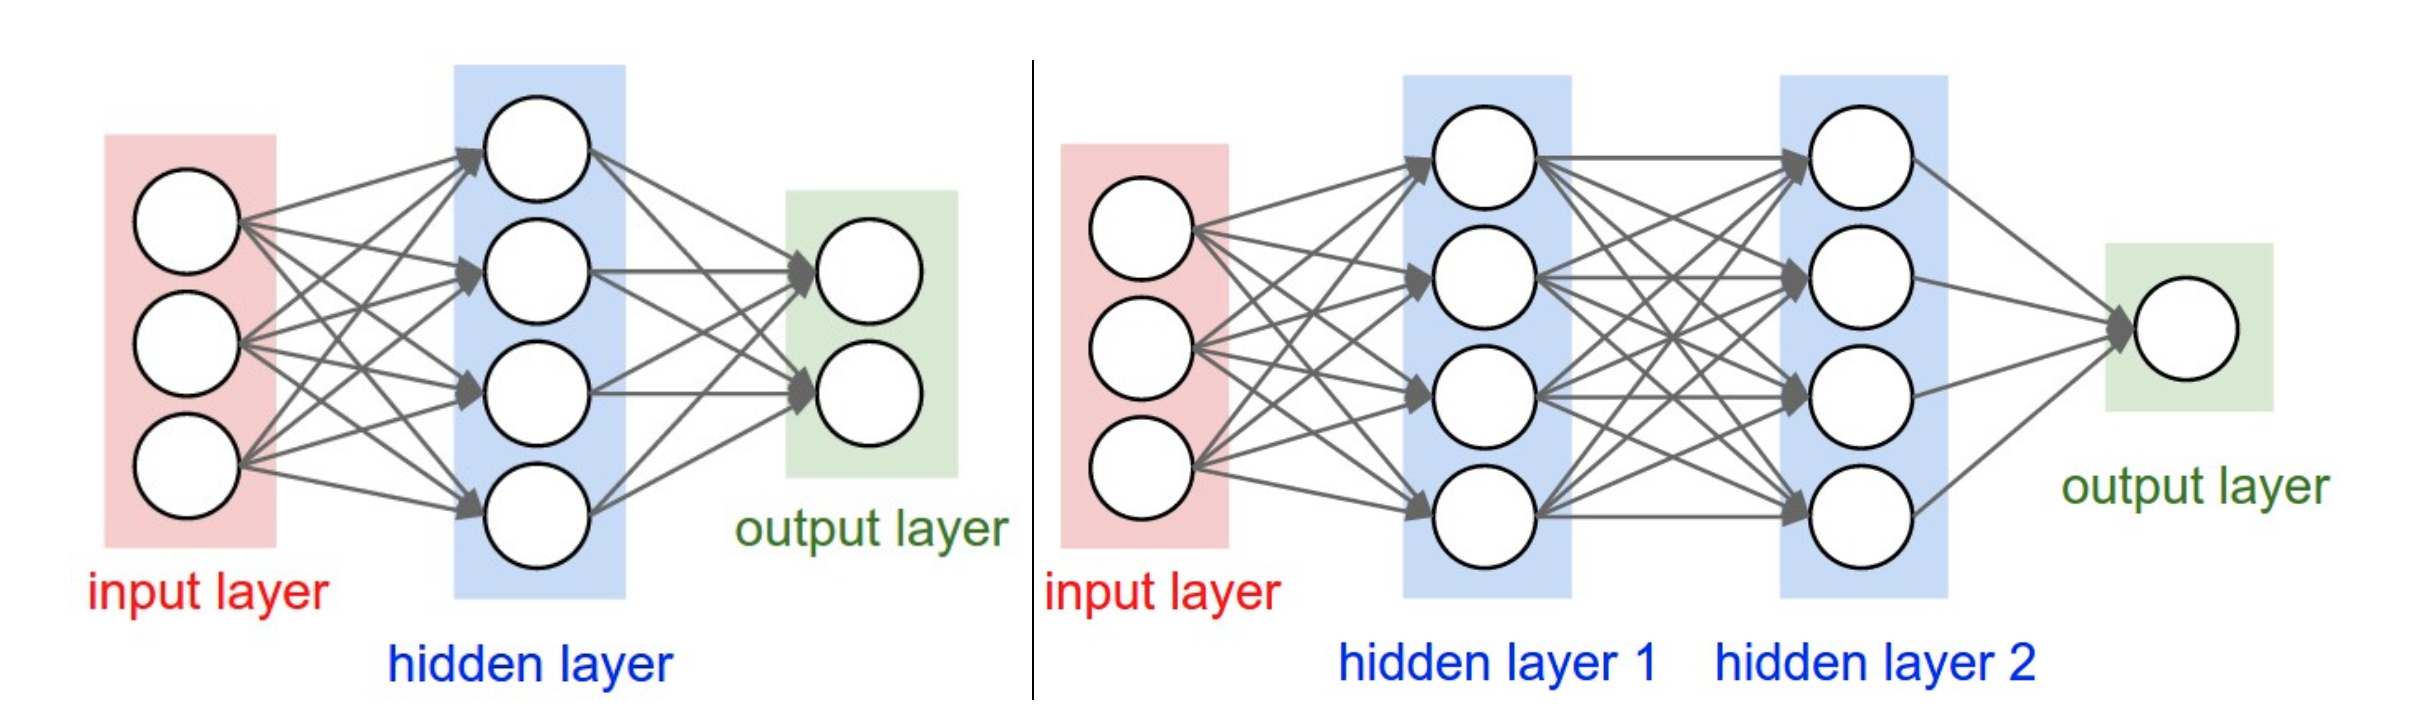
\includegraphics[scale=0.35]{chapter3/MLP}
  \label{fig:MLP}
\end{figure}

\section{CNN}

What is the architecture of CNNs`?

\section{AlexNet}

\section{Inception}

Explain Inception and why it's so amazing

\section{ResNet}

Explain Resnet and why it's so amazing
